\documentclass[tikz,dvisvgm]{standalone}

\usetikzlibrary{calc,positioning,shapes.multipart,shapes.misc,chains,arrows}
\usepackage{xcolor}
\colorlet{myred}{red!80!black}

\begin{document}

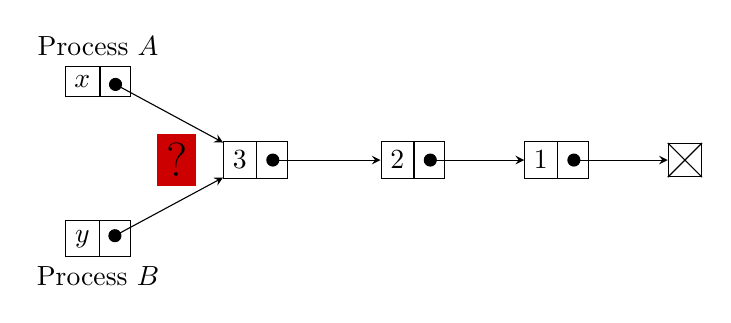
\begin{tikzpicture}[list/.style={rectangle split, rectangle split parts=2,
  draw, rectangle split horizontal}, >=stealth, start chain, distance=5mm and 5mm]

  \node[list,on chain] (A) {3};
  \node[list, on chain,label=Process $A$](P1) [above of=A,xshift=-30mm] {$x$};
  \node[list, on chain,label=below:Process $B$](P2) [below of=A,xshift=-30mm] {$y$};
  \node (dot) [left of=A,font=\LARGE,fill=myred] {?}; 
  \node[list,on chain] (B) [right of=A] {2};
  \node[list,on chain] (C) {1};
  \node[on chain,draw,inner sep=6pt] (D) {};
  \draw (D.north east) -- (D.south west);
  \draw (D.north west) -- (D.south east);
  \draw[*->] let \p1 = (A.two), \p2 = (A.center) in (\x1,\y2) -- (B);
  \draw[*->] let \p1 = (B.two), \p2 = (B.center) in (\x1,\y2) -- (C);
  \draw[*->] let \p1 = (C.two), \p2 = (C.center) in (\x1,\y2) -- (D);
  \draw[*->] let \p1 = (P1.two), \p2 = (P1.center) in (\x1,\y2) -- (A);
  \draw[*->] let \p1 = (P2.two), \p2 = (P2.center) in (\x1,\y2) -- (A);

\end{tikzpicture}

\end{document}